% app1.tex (file to switch to appendix mode)
\newpage

\invisiblechapter{\violinPiece}

\vspace{3.8cm}

\begin{center}

\textsc{for solo violin}

\vspace{2.8cm}

\HRule{0.5pt}

\LARGE \textbf{\uppercase{\violinPiece}}

\HRule{2pt}

\vspace{1.8cm}

\normalsize \today

\vspace{3.8cm}

Rhys Gray

\end{center}
\newpage
\section*{Program Notes}
\violinPiece is a solo work for violin that explores half-harmonics.
It is a non-programmatic work, and the title was inspired by a question that my supervisor posed to me while I sought ethics approval for my exegesis; a simple phrase laden with possible contexts, spurring the imagination to try and complete the meaning.

It is, in a way, an etude that explores half-harmonics, similar to those found in Sciarrino's \emph{6 Caprricio for violin}. 
Half-harmonics are produced by applying left hand finger pressure halfway between that required to create a harmonic, and a \emph{normale} sound. 
The sound that is produced should be a mixture of the stopped string pitch, the harmonic pitch, and a resistant, slightly noisy quality.

\section*{Notation}
\begin{itemize}

    \item Half-harmonics are notated in the score as a half-filled diamond notehead.
    \item sp denotes \emph{sul ponticello}.
    \item msp denotes \emph{molto sul ponticello}.
    \item similarly, st denotes \emph{sul tasto}, and mst denotes \emph{molto sul tasto}
\end{itemize}

\newpage

% 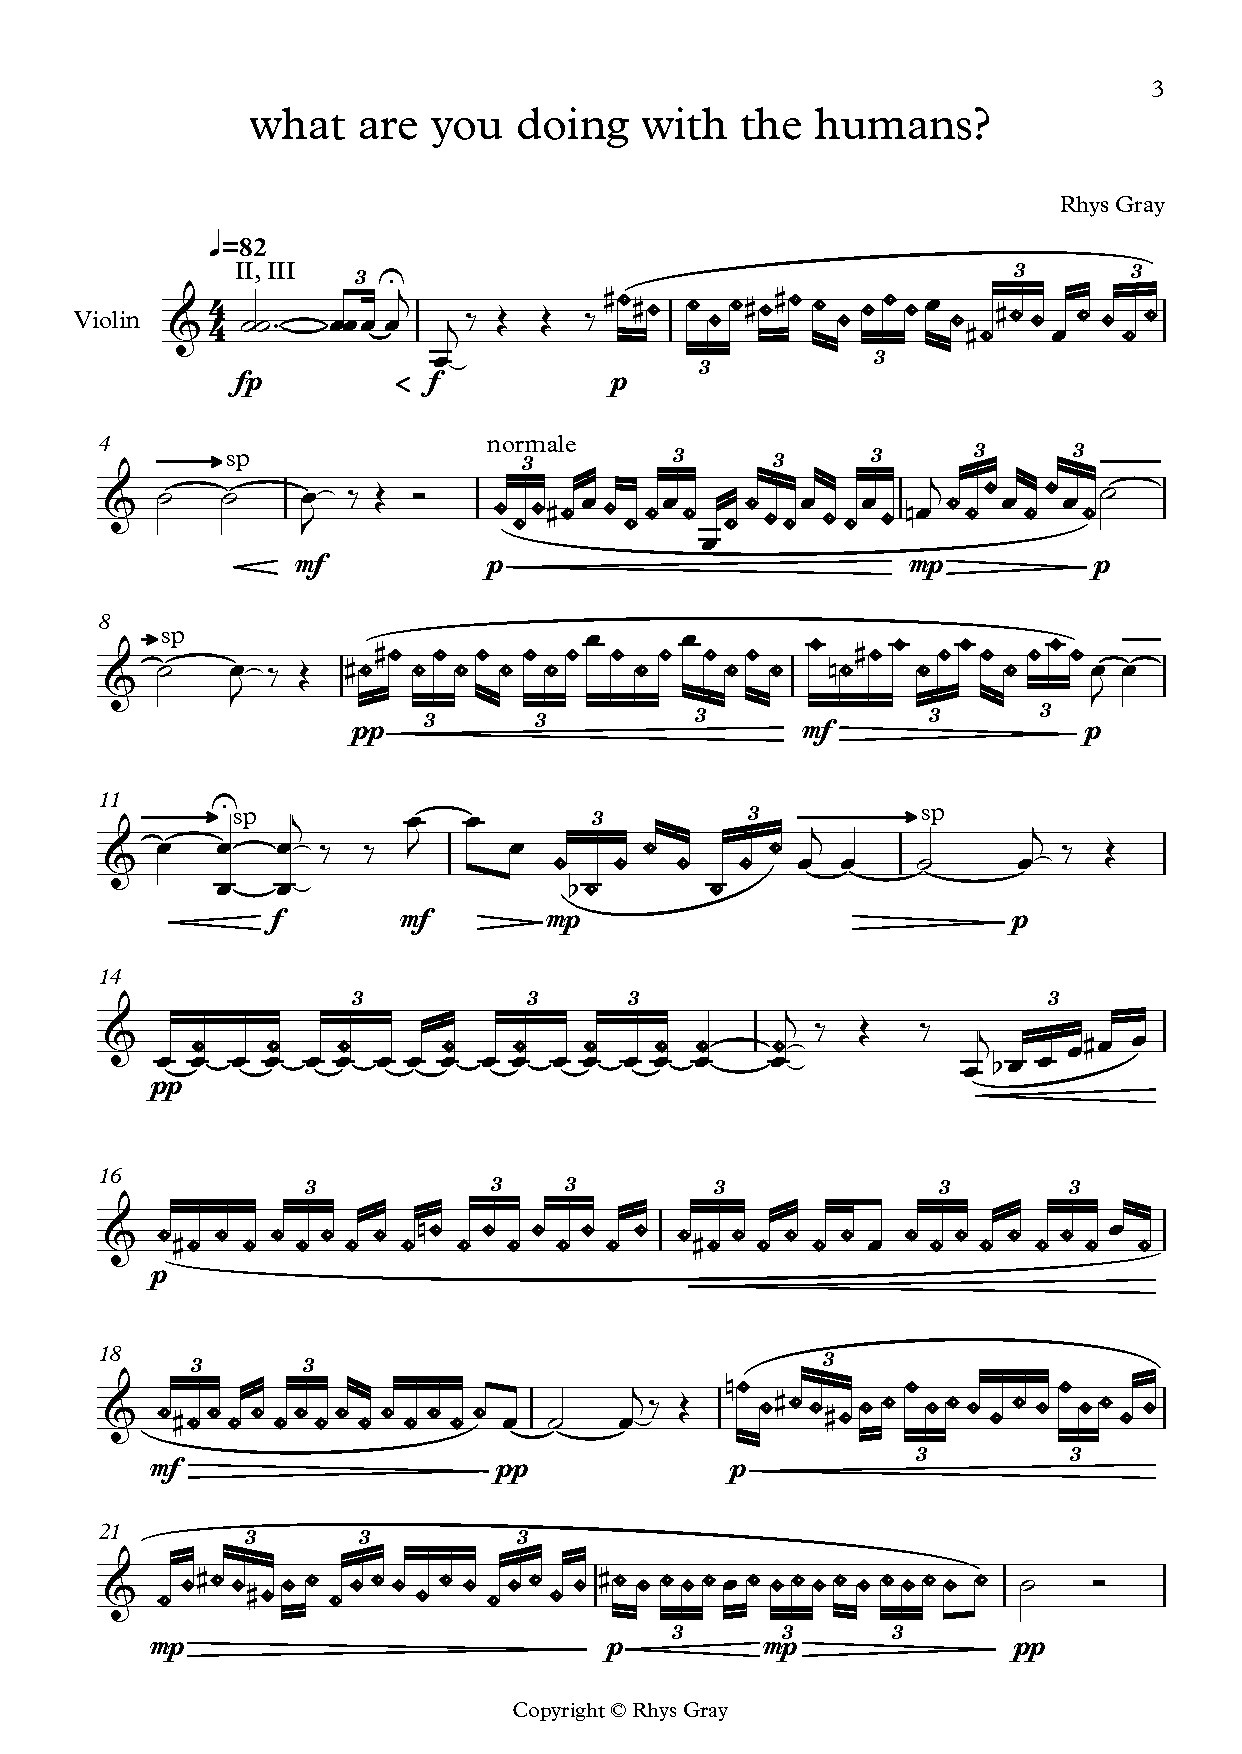
\includepdf[pages=-,pagecommand={},width=\textwidth]{resources/compositions/violin.pdf}

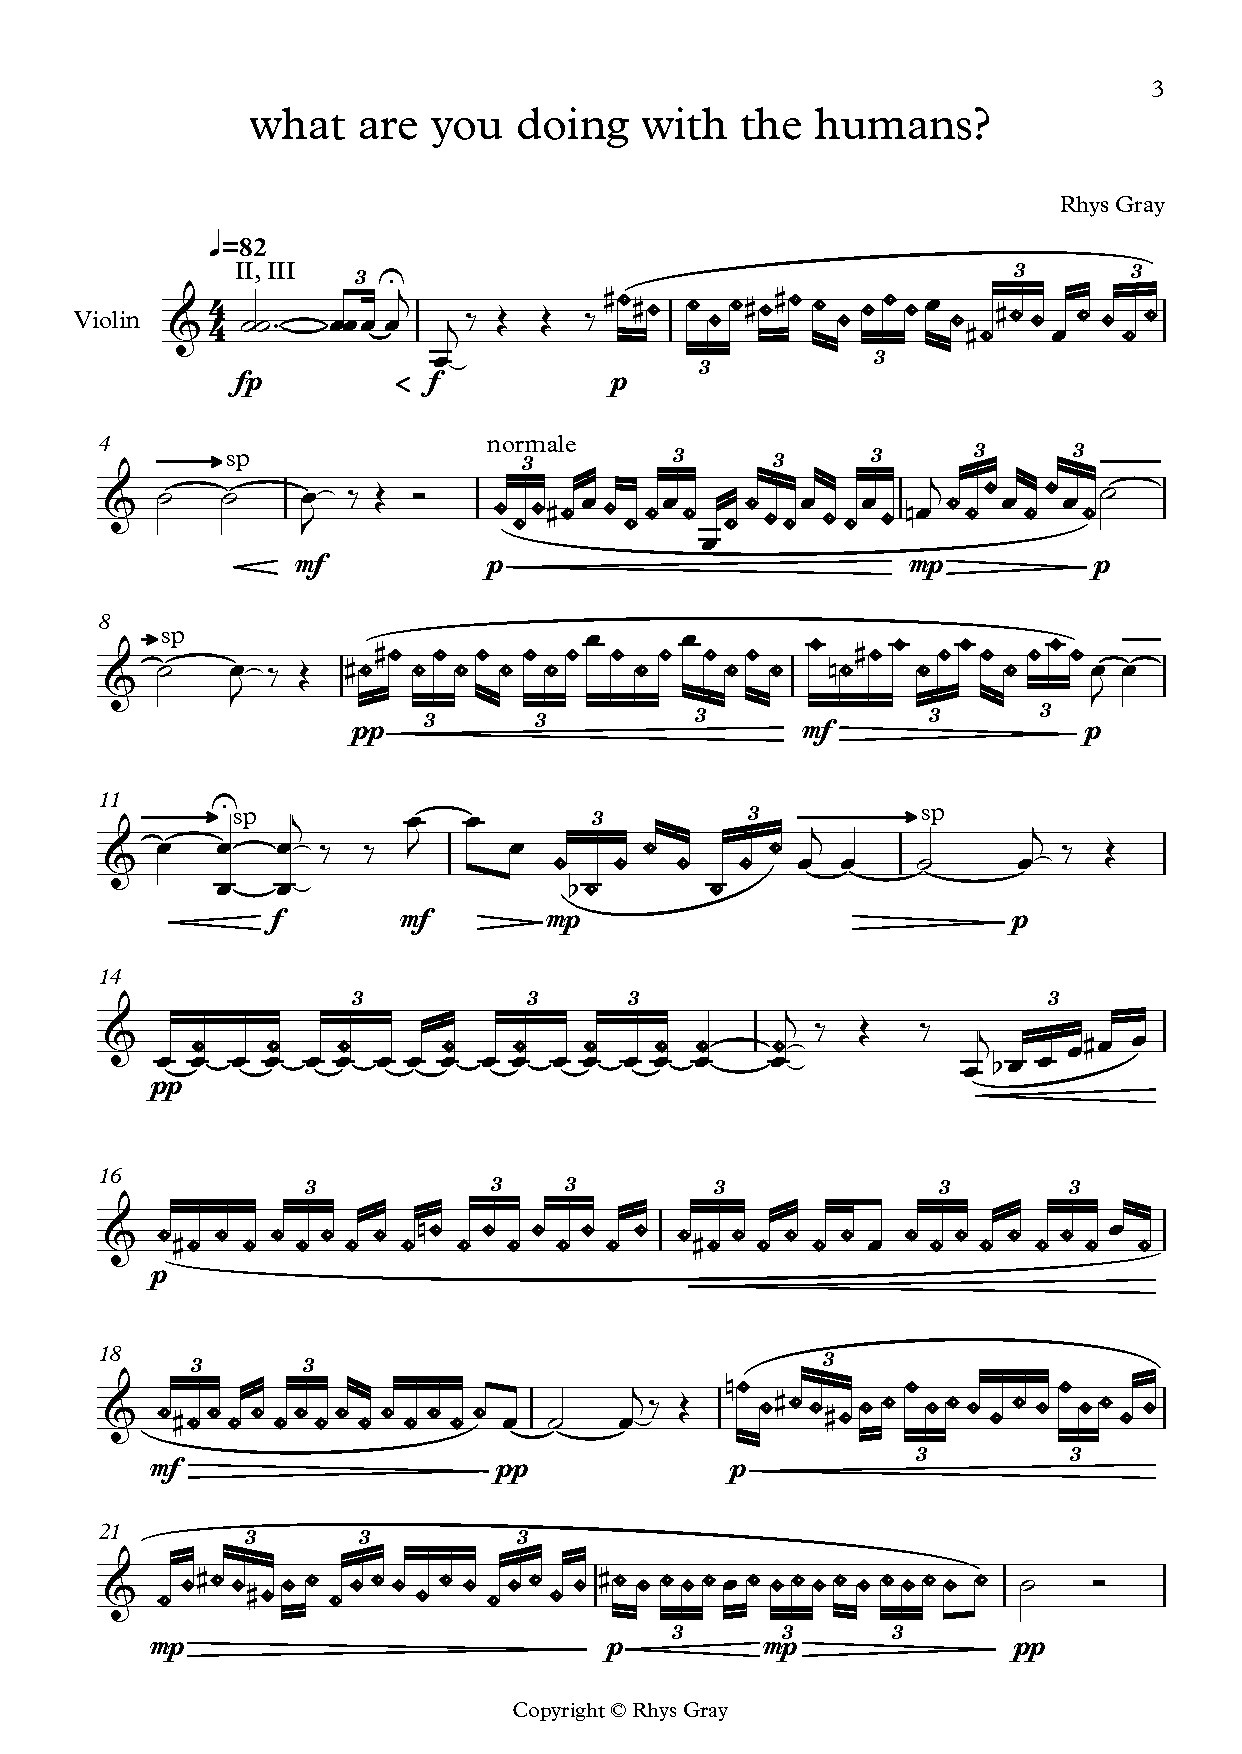
\includepdf[pages=-,pagecommand={}]{resources/compositions/violin.pdf}